\documentclass[letterpaper]{amsart}
\usepackage{amsmath, amsthm, amsfonts, amsbsy, thmtools, amssymb,bm,xfrac,stmaryrd,mathrsfs,bbm}
\usepackage{tikz}
\usetikzlibrary{arrows}

\begin{document}

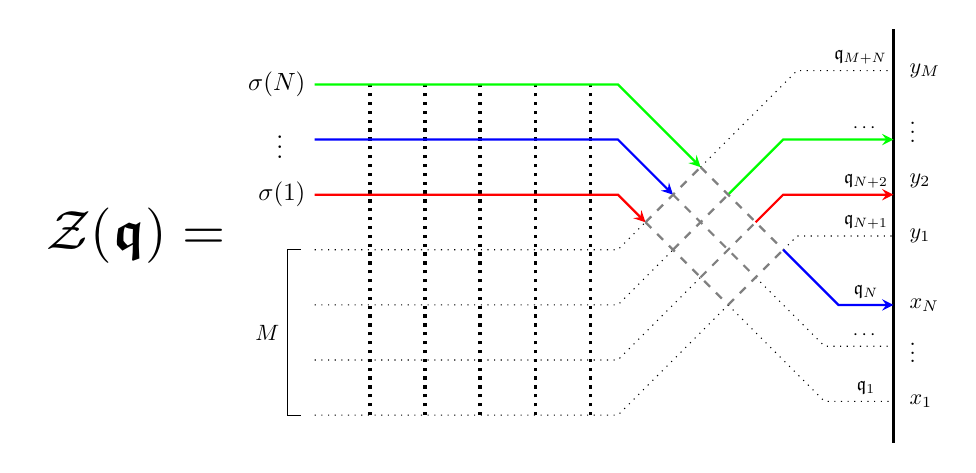
\begin{tikzpicture}[
	>=stealth, 
	scale = .7]{
		\draw[-, very thick] (9, -.5) -- (9, 7);

		\draw[very thick, dotted] (-.5, 0) -- (-.5, 6);
		\draw[very thick, dotted] (.5, 0) -- (.5, 6);
		\draw[very thick, dotted] (1.5, 0) -- (1.5, 6);
		\draw[very thick, dotted] (2.5, 0) -- (2.5, 6);
		\draw[very thick, dotted] (3.5, 0) -- (3.5, 6);

		\draw[] (-4.75, 3.25) circle [radius = 0] node[scale=2]{$\mathcal{Z} (\bm{\mathfrak{q}}) = $};
		\draw[dotted] (7, 3) -- (7.25, 3.25) -- (9, 3.25) node[right = 3, scale = .8]{$y_1$};
		\draw[] (9, 4.25) circle [radius = 0] node[right = 3, scale = .8]{$y_2$};
		\draw[]  (9, 5.25)circle [radius = 0] node[right = 3, scale = .8]{$\vdots$};
		\draw[dotted] (5.5, 4.5) -- (7.25, 6.25) -- (9, 6.25) node[right = 3, scale = .8]{$y_M$};

		\draw[dotted] (6, 2) -- (7.75, .25) -- (9, .25) node[right = 3, scale = .8]{$x_1$};
		\draw[dotted] (6.5, 2.5) -- (7.75, 1.25) -- (9, 1.25) node[right = 3, scale = .8]{$\vdots$};
		\draw[]  (9, 2) circle [radius = 0] node[right = 3, scale = .8]{$x_N$};

		\draw[->, red, thick] (-1.5, 4) node[left, black, scale = .9]{$\sigma(1)$} -- (4, 4) -- (4.5, 3.5);
		\draw[->, blue, thick] (-1.5, 5) node[left = 8, black, scale = .9]{$\vdots$} -- (4, 5) -- (5, 4); 
		\draw[->, green, thick] (-1.5, 6) node[left, black, scale = .9]{$\sigma(N)$} -- (4, 6) -- (5.5, 4.5);

		\draw[dotted] (-1.5, 0) -- (4, 0) -- (6, 2);
		\draw[dotted] (-1.5, 1) -- (4, 1) -- (5.5, 2.5);
		\draw[dotted] (-1.5, 2) -- (4, 2) -- (5, 3);
		\draw[dotted] (-1.5, 3) -- (4, 3) -- (4.5, 3.5);


		\draw[gray, dashed, thick] (4.5, 3.5) -- (5.5, 4.5); 
		\draw[gray, dashed, thick] (6, 2) -- (7, 3); 
		\draw[->, thick, red] (6.5, 3.5) -- (7, 4) -- (9, 4); 
		\draw[gray, dashed, thick] (5.5, 2.5) -- (6.5, 3.5); 
		\draw[->, thick, green] (6, 4) -- (7, 5) -- (9, 5); 
		\draw[gray, dashed, thick] (5, 3) -- (6, 4);

		\draw[gray, dashed, thick] (4.5, 3.5) -- (6, 2);
		\draw[gray, dashed, thick] (5, 4) -- (6.5, 2.5);
		\draw[gray, dashed, thick] (5.5, 4.5) -- (7, 3); 
		\draw[->, thick, blue] (7, 3) -- (8, 2) -- (9, 2);

		\draw[-] (-1.75, 0) -- (-2, 0) -- (-2, 3) -- (-1.75, 3);
		\draw[] (-2, 1.5) circle [radius = 0] node[left, scale = .8]{$M$};

		\draw[] (8.5, .25) circle [radius = 0] node[above, scale = .7]{$\mathfrak{q}_1$};
		\draw[] (8.5, 1.25) circle [radius = 0] node[above, scale = .7]{$\cdots $};
		\draw[] (8.5, 2) circle [radius = 0] node[above, scale = .7]{$\mathfrak{q}_N$};
		\draw[] (8.5, 3.25) circle [radius = 0] node[above, scale = .7]{$\mathfrak{q}_{N+1}$};
		\draw[] (8.5, 4) circle [radius = 0] node[above, scale = .7]{$\mathfrak{q}_{N+2}$};
		\draw[] (8.5, 5) circle [radius = 0] node[above, scale = .7]{$\cdots$};
		\draw[] (8.4, 6.25) circle [radius = 0] node[above, scale = .7]{$\mathfrak{q}_{M+N}$};

	}
\end{tikzpicture}

\end{document}